\documentclass[border=6pt,tikz]{standalone}
\usepackage{tikz}
\usepackage{amsmath,amssymb}
\usetikzlibrary{arrows.meta,positioning,fit,backgrounds,calc,shapes.geometric,decorations.pathreplacing,patterns}
\definecolor{ink}{HTML}{1B2430}
\definecolor{muted}{HTML}{6B7785}
\definecolor{accent}{HTML}{2F6FB5}
\definecolor{accent2}{HTML}{C1611F}
\definecolor{good}{HTML}{2E7D5B}
\definecolor{soft}{HTML}{EDF2F7}
\definecolor{soft2}{HTML}{FBEDE2}
\definecolor{soft3}{HTML}{E6F0E9}
\tikzset{
  box/.style={draw=ink,line width=.7pt,rounded corners=2pt,fill=soft,inner sep=4pt,align=center,font=\sffamily\small},
  boxa/.style={box,fill=soft2},
  boxb/.style={box,fill=soft3},
  plain/.style={align=center,font=\sffamily\small,text=ink},
  tiny/.style={align=center,font=\sffamily\scriptsize,text=muted},
  ar/.style={-{Stealth[length=2.4mm]},draw=ink,line width=.7pt},
  arm/.style={-{Stealth[length=2.4mm]},draw=muted,line width=.6pt,dashed},
  nd/.style={circle,draw=ink,line width=.7pt,fill=white,minimum size=7mm,inner sep=0pt,font=\sffamily\scriptsize},
  ndf/.style={nd,fill=soft},
  ndt/.style={nd,fill=soft2},
}

\begin{document}
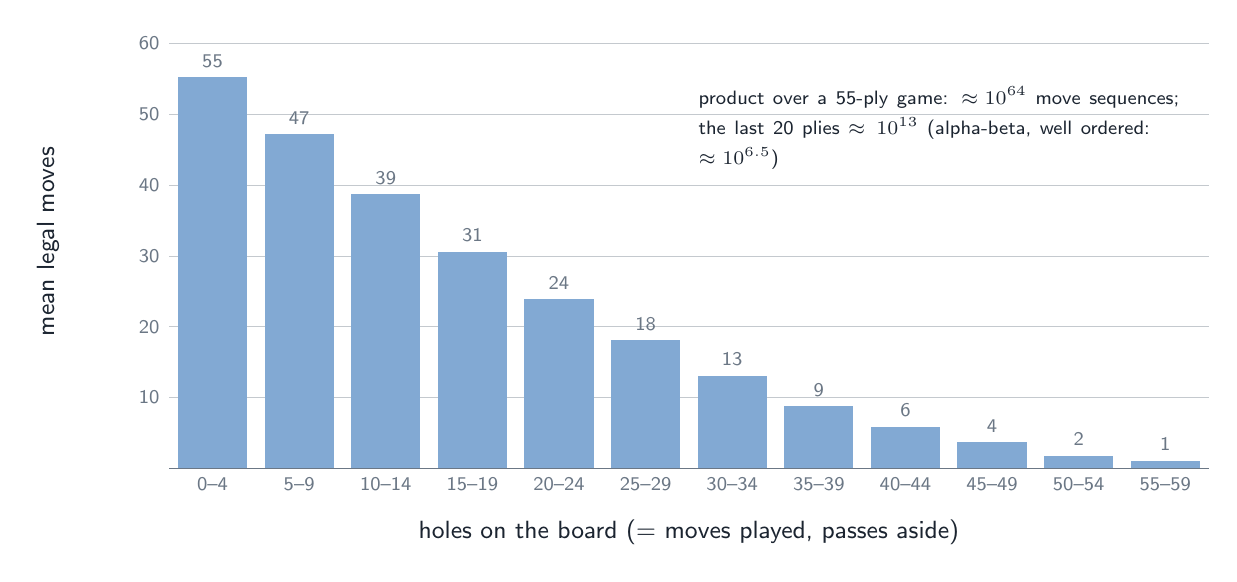
\begin{tikzpicture}[x=2.2mm,y=0.9mm]
\draw[muted,line width=.3pt] (0,0) -- (60,0);
\draw[muted!40,line width=.2pt] (0,10) -- (60,10); \node[tiny,left] at (0,10) {10};
\draw[muted!40,line width=.2pt] (0,20) -- (60,20); \node[tiny,left] at (0,20) {20};
\draw[muted!40,line width=.2pt] (0,30) -- (60,30); \node[tiny,left] at (0,30) {30};
\draw[muted!40,line width=.2pt] (0,40) -- (60,40); \node[tiny,left] at (0,40) {40};
\draw[muted!40,line width=.2pt] (0,50) -- (60,50); \node[tiny,left] at (0,50) {50};
\draw[muted!40,line width=.2pt] (0,60) -- (60,60); \node[tiny,left] at (0,60) {60};
\fill[accent!60] (0.5,0) rectangle (4.5,55.2);
\node[tiny,above] at (2.5,55.2) {55};
\node[tiny,below] at (2.5,0) {0--4};
\fill[accent!60] (5.5,0) rectangle (9.5,47.2);
\node[tiny,above] at (7.5,47.2) {47};
\node[tiny,below] at (7.5,0) {5--9};
\fill[accent!60] (10.5,0) rectangle (14.5,38.7);
\node[tiny,above] at (12.5,38.7) {39};
\node[tiny,below] at (12.5,0) {10--14};
\fill[accent!60] (15.5,0) rectangle (19.5,30.6);
\node[tiny,above] at (17.5,30.6) {31};
\node[tiny,below] at (17.5,0) {15--19};
\fill[accent!60] (20.5,0) rectangle (24.5,23.9);
\node[tiny,above] at (22.5,23.9) {24};
\node[tiny,below] at (22.5,0) {20--24};
\fill[accent!60] (25.5,0) rectangle (29.5,18.1);
\node[tiny,above] at (27.5,18.1) {18};
\node[tiny,below] at (27.5,0) {25--29};
\fill[accent!60] (30.5,0) rectangle (34.5,13.1);
\node[tiny,above] at (32.5,13.1) {13};
\node[tiny,below] at (32.5,0) {30--34};
\fill[accent!60] (35.5,0) rectangle (39.5,8.8);
\node[tiny,above] at (37.5,8.8) {9};
\node[tiny,below] at (37.5,0) {35--39};
\fill[accent!60] (40.5,0) rectangle (44.5,5.9);
\node[tiny,above] at (42.5,5.9) {6};
\node[tiny,below] at (42.5,0) {40--44};
\fill[accent!60] (45.5,0) rectangle (49.5,3.7);
\node[tiny,above] at (47.5,3.7) {4};
\node[tiny,below] at (47.5,0) {45--49};
\fill[accent!60] (50.5,0) rectangle (54.5,1.8);
\node[tiny,above] at (52.5,1.8) {2};
\node[tiny,below] at (52.5,0) {50--54};
\fill[accent!60] (55.5,0) rectangle (59.5,1.1);
\node[tiny,above] at (57.5,1.1) {1};
\node[tiny,below] at (57.5,0) {55--59};
\node[plain] at (30,-9) {holes on the board (= moves played, passes aside)};
\node[plain,rotate=90] at (-7,32) {mean legal moves};
\node[plain,anchor=west,text width=62mm,align=left] at (30,48) {\scriptsize product over a 55-ply game: $\approx 10^{64}$ move sequences;\\ \scriptsize the last 20 plies $\approx 10^{13}$ (alpha-beta, well ordered: $\approx 10^{6.5}$)};
\end{tikzpicture}
\end{document}
